\prob
{
    Let $T_8$ and $R_8$ be matroids in [\ref{t2:p7}]. Give geometric
		representations for each of $T_8 / 8$, $T_8 / 1$, $R_8 / 8$ and $R_8 / 1$.
}
\begin{proof}
    The only interesting case is $T_8 / 8$. $T_8 / 1$ will be exactly the same case as in [\ref{t2:p7_T8DualMinorGraphicRepresentation.png}] 
    (which is the representation of $F_7^-$) with a posible relabeling of the points. As every point in $R_8$ does behave exactly the same, 
    it doesn't matter if you contract $8$ or $1$, the result will be completely analog to the one in 
    [\ref{t2:p7_R8DualMinorGraphicRepresentation.png}] (which is again the representation of $F_7^-$).
    
    The case of $T_8 / 8$ is only one that we have not seen yet. 
    
    \begin{figure}[H]
        \begin{center}
            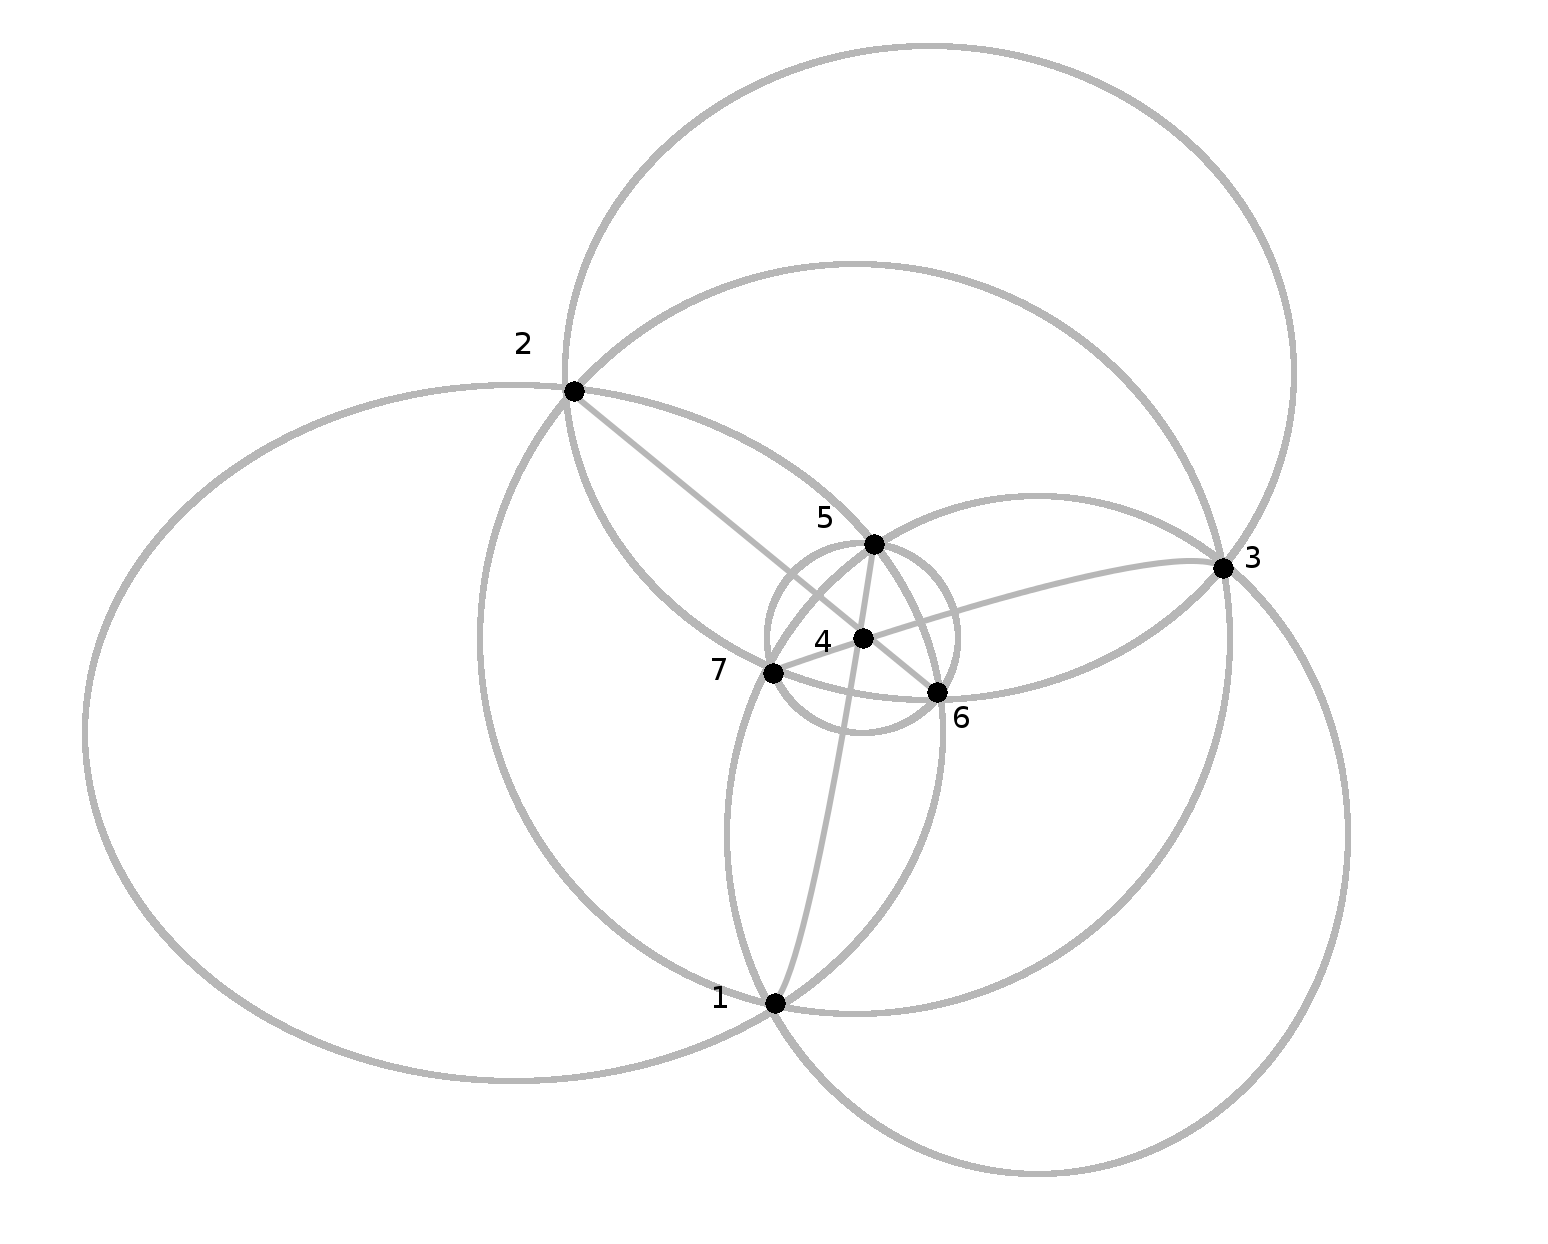
\includegraphics[width=8cm]{Test2/Problem17/T8_contracting_8.png}
        \end{center}                            
        \caption{Geometric representation for $T_8 / 8$}
        \label{t2:p17_T8_contracting_8.png}                        
    \end{figure}\pn  
\end{proof}